\section{Technique}
\label{sec:technique}

The main objectives of the proposed visualization were:

\begin{enumerate}
\item to give a panoramic macro view of the evolution of EC number annotations
\item to allow users to explore the complete set of changes, including entry metadata, formulating and answering general questions about EC number changes
\end{enumerate}

Concerning the first objective, we wanted to present in a single perspective the EC changes segmented by all the possible combinations of events, considering the three parameters of the model (common prefix length, number of generalizations and specializations) across all the database releases.

\subsection{Multivariate display}

We have a multivariate problem where the fundamental task is to compare multiple instances of several variables at once and to allow users to identify similarities and differences among them. Small Multiples of Tufte  \cite{tufte_envisioning} or Trellis Displays of Cleveland \cite{cleveland_trellis1,cleveland_trellis2} are a straightforward approach to present our data. They consist of splitting the data into multiple graphs that are presented close to each other in the screen allowing easier examination of the data in a given graph, and comparison of values and patterns among graphs to be relatively simple.
 
According to Few \cite{few_nysi}, individual graphs display a subset of a dataset originally divided according to a categorical variable and the several graphs differ only in terms of the data being displayed. Every graph ideally shares the same type, shape, and size and, consequently the same categorical and quantitative scales. Scales in each graph must start and end with the same values (otherwise the accurate comparison is more difficult). Graphs can be arranged horizontally or vertically or as a matrix in a meaningful order. 

\subsubsection{Basic frame}

With that in mind, we proceed our explanation of the proposed visual representation. The basic graph of the proposed Small Multiple representation, which we call from now on \textit{frame}, is presented in Figure \ref{fig:technique}. It is a two dimensional plot where we present in the x-axis the number of specializations and in the y-axis, the number of generalizations. Both x and y-axes vary in the interval [0,4].

Notice some remarkable positions in the frame:

\begin{description}
\item [Position (0,0):] entries with no changes in the corresponding pair of versions.
\item [Diagonal:] entries which suffered the same level of generalizations and specializations, potentially error corrections. They are presented in beige in Quadmap.
\item [Lower right matrix:] entries that suffered more levels of specializations than generalizations, in other words, knowledge about the catalyzed reaction has increased. They are presented in blue in Quadmap.
\item [Upper left matrix:] entries that suffered more levels of generalizations than specializations, in other words, knowledge about catalyzed reaction has decreased. They are presented in red in Quadmap.
\item [Invalid positions: ] if a change keeps a common prefix of size 3, it is impossible to have 2 degrees of generalization. Events like this are presented in a darker shade of gray.
\end{description}

\begin{figure}[htb]
  \centering
  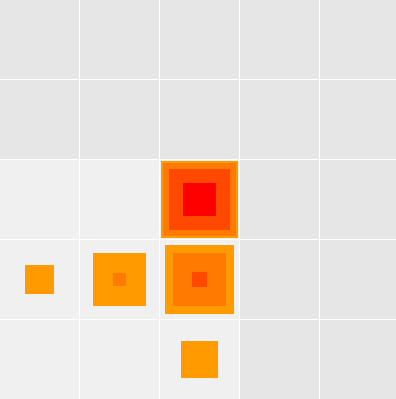
\includegraphics[width=3.7cm]{images/techniquea.png} (a) 
  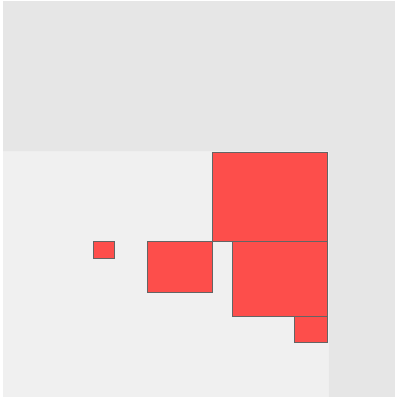
\includegraphics[width=3.7cm]{images/techniqueb.png} (b)
  \caption{Basic frames for the proposed small multiple visualization. In (a), we present the Heatmap version and in (b), the Quadmap. In (a),  the darker the green, the higher the value represented. Likewise, in (b), the bigger the rectangle area, the higher the value. Red represents entries which presented more levels of generalizations than specializations, in other words, points above the diagonal. In blue, we present the points with more levels of specializations than generalizations, that means, points bellow  the diagonal. Finally, in beige, we represent diagonal points which present the same levels of generalizations and specializations.}
  \label{fig:technique}
\end{figure}

Several frames like the one shown are then arranged in a Small Multiple fashion as in Figure \ref{fig:heatmap000}. In x-axis, we represent the consecutive pairs of released versions. The y-axis presents the possible common prefixes in [0,4]. 

\begin{figure*}[htb]
  \centering
  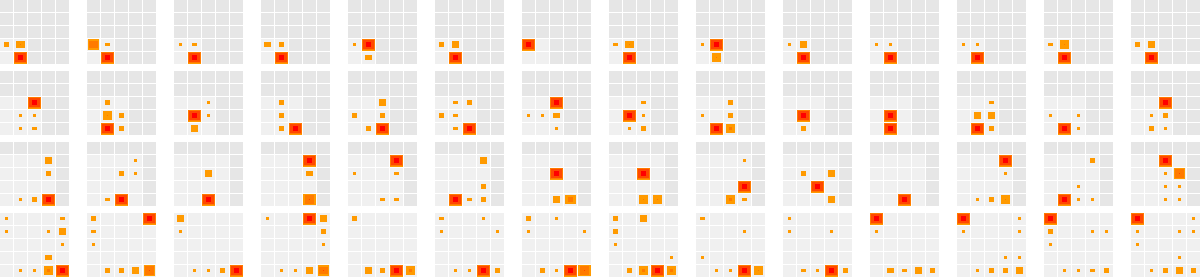
\includegraphics[width=17cm]{images/heatmap000.png}
  \caption{Multivariate view with Heatmaps.}
  \label{fig:heatmap000}
\end{figure*}

\subsubsection{Heatmap}
\label{heatmap}

In a first version of the graph, we use a Heatmap representation where color is a pre-attentive attribute that encodes the frequency of a given change configuration. 

The aim of this representation was to bring forth an overview of the complete data, evidencing trends and exceptions across the 15 releases. An interesting feature of this representation is that values in the lower right triangular matrix represents specializations and in the upper left triangular matrix, generalizations. Consequently, it is easy to recognize global trends towards generalization or specialization in enzyme reaction annotations.

\subsubsection{Quadmap}
\label{quadmap}

Heatmaps present relevant trends in terms of generalization and specialization occurrences but we see two possible drawbacks in that approach. 

Firstly, color is not a pre-attentive attribute able to precisely encode quantitative data. Most certainly, one can perceive that an intense color represents a higher value than a less intense one. However, it is very difficult to precisely estimate the values from color intensities. 

The second drawback is that our heatmap presents too much blank space. According to Tufte \cite{tufte_envisioning}, the data density of a graph is the proportion of the total size of the graph that is dedicated to displaying data. Tufte prefers high data density graphs as the human perceptual system is capable of detecting subtle patterns, trends and exceptions. On account of that, we decided to propose a second, complementary view, hoping to reduce blank (non-data) space and also improve quantity estimation. 

The Quadmap representation was inspired in two-dimensional scatter plots where the points are rectangles with its area representing frequency. Even though area is not the most precise visual attribute to encode quantity, it is more precise than colors. Notice, in Figure \ref{fig:technique}, that it is easier to estimate quantities in the Quadmap (b) than in the Heatmap (a).

It is important to highlight that in Quadmaps axes are different from one frame to the other, going against the rule of axis and scale preserving in Small Multiples. This happens because rectangle sizes distort tics in axes. Nevertheless, we believe this option helps to emphasize trends and exceptions by using colored pixels to represent quantities more precisely than in Heatmaps.

\subsection{Analytical interaction and navigation}

\subsubsection{Filtering, scales and normalization options}

The efficaciousness of the information visualization techniques hinge on their ability to clearly and accurately represent information and on the capacity to fathom underlying information through interaction. Indeed, no matter how rich the display is, questions will arise, making interaction a necessary instrument in the pursuit of answers. Furthermore, contrasting different perspectives can lead to different insights. The proposed visualization provides pre-defined filters and different scaling and normalization options: 

\begin{enumerate}
\item \textbf{Logarithmic scale on the frequencies:} rectangle area or heatmap colors are computed according to a logarithmic scale of frequencies
\item \textbf{Normalization of frequencies globally or by frame:} global normalization leads to a more realistic view of frequencies while local (or frame) normalization, despite contradicting Small Multiple rules, emphasizes a part-to-whole relationship into a give frame.
\item \textbf{Filter by only changes or presentation of the complete data set}: data is very unbalanced as we have much more stable entries than changes. In conclusion, when we exhibit the complete dataset, the changes are de-emphasized. 
\end{enumerate}

\subsubsection{Hierarchical navigation}

A particularly interesting way to create dense graphics is through what Tufte calls micro/macro readings \cite{tufte_envisioning}. These graphics convey one layer of information on a micro scale and another layer on a zoomed out, macro scale. A nice consequence of this technique is that information is consumed hierarchically. The viewer may glance from the distance to observe a global trend and, later, peer closely to examine individual pieces of that trend. Our multivariate view is a macro view of the whole set of changes in the dataset. Users can click on each frame and see it zoomed in a micro view. In other words, as seen in Figure \ref{fig:navigation}, users can select a specific release and common prefix length and view a detailed description of the respective frame.

Additionally, users can click on the points in the micro view and see interactive histograms of each type of change. Through these histograms users can see the enzyme families which have suffered that change. These histograms are composed by small rectangles representing each change and by clicking on individual rectangles users can see details about that specific entry. 

\begin{figure*}[htb]
  \centering
  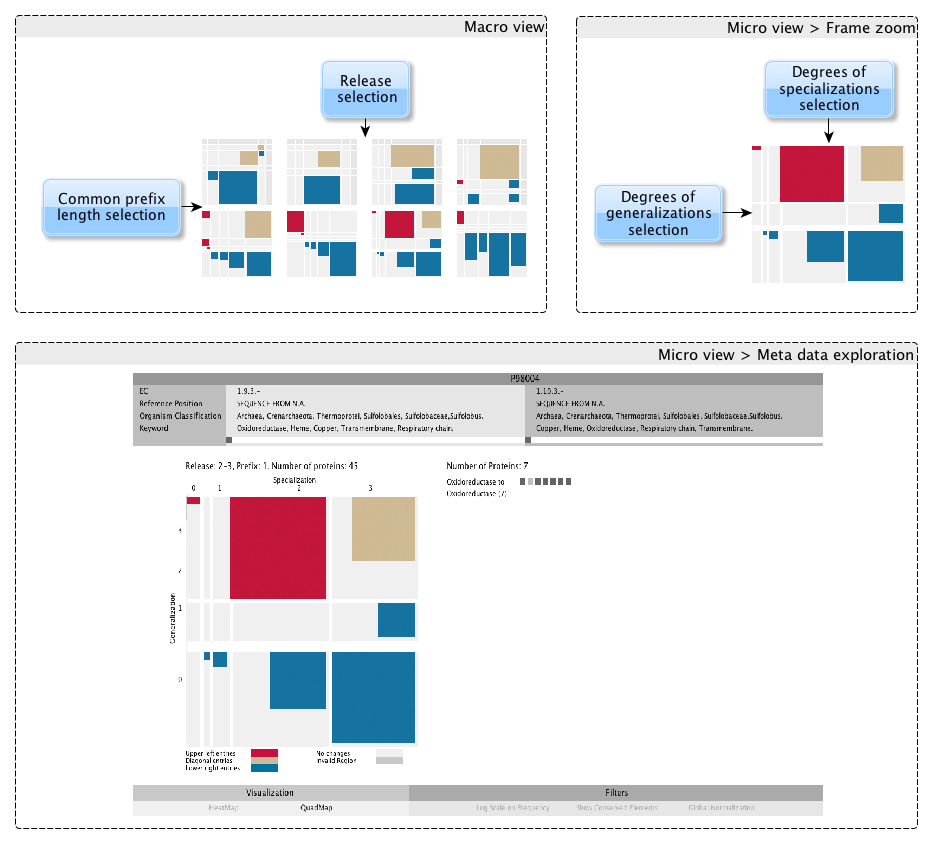
\includegraphics[width=17cm]{images/navigation2.png} 
  \caption{Navigation scheme.}
  \label{fig:navigation}
\end{figure*}
